\chapter{Поле 203: вид содержания, средства доступа, характеристика содержания}

Поле введено в ИРБИС64+ версии 2018.1 в связи с переходом на ГОСТ 7.0.100-2018.

\begin{figure}
    \centering
    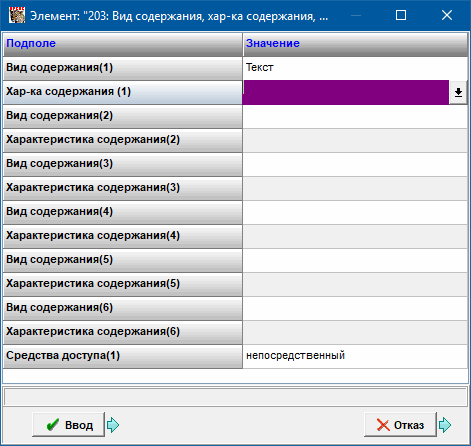
\includegraphics[width=0.7\linewidth]{img/field203}
    \caption[Вложенный рабочий лист для поля 203]{Вложенный рабочий лист для поля 203}
    \label{fig:field203}
\end{figure}

Поле соответствует Области вида содержания и средства доступа ГОСТ Р 7.0.100-2018, назначение которой -- предоставить сведения о природе информации, содержащейся в ресурсе, и средстве, обеспечивающем доступ к нему, чтобы помочь пользователям каталога в идентификации и выборе ресурсов, соответствующих их потребностям.

Поле факультативное. Повторяется, если использование ресурса возможно с помощью различных средств доступа.

\section{Подполя A, B, D, E, F, G, I, K, L: вид содержания}

Категории вида содержания отражают основной вид информации, имеющейся в ресурсе. В подполе следует использовать термины из перечня терминов, определенных в ГОСТ Р 7.0.100-2018 для элемента "<Вид содержания">.

Подполе обязательное, если поле 203 присутствует в записи. В ИРБИС64 предусмотрено до 6 повторений подполя (распределено по подполям A, B, D, E, F, G, I, K, L).

Значения берутся из справочника \emph{vso.mnu}.

\begin{cutelist}
    \item Движение
    \item Звуки
    \item Изображение
    \item Музыка
    \item Предмет
    \item Текст
    \item Устная речь
    \item Электронная программа
    \item Электронные данные
\end{cutelist}

\section{Подполя C, 1, 2, 3, 4, 5, 6, 7, 8: средство доступа }

Средство доступа характеризует возможности хранения, использования или передачи содержания ресурса как с помощью специализированных устройств (аппаратов), так и без них. В подполе следует использовать термины из перечня терминов, определенных в ГОСТ Р 7.0.100-2018 для элемента "<Средство доступа">. Термины средства доступа приводят в грамматическом согласовании с терминами вида содержания и характеристики содержания.

Подполе обязательное, если поле 203 присутствует в записи. Не повторяется.

Значения берутся из справочника \emph{tso.mnu}.

\begin{cutelist}
    \item аудио
    \item видео
    \item микроскопический
    \item микроскопическое
    \item микроформа
    \item непосредственный
    \item непосредственное
    \item проекционный
    \item проекционное
    \item стереографический
    \item стереографическое
    \item электронный
    \item электронное
    \item электронная
    \item электронные
    \item разные средства доступа
    \item другое средство доступа
\end{cutelist}

\section{Подполя O, P, U, Y, T, R, W, Q, X, V, Z: характеристика содержания}

Категория вида содержания может быть дополнена одним или несколькими терминами характеристики содержания, которые применимы к описываемому ресурсу. Характеристики содержания уточняют природу информации, способ сенсорного восприятия, наличие или отсутствие движения, размерность объекта описания. В подполе следует использовать термины из перечня терминов, определенных в ГОСТ Р 7.0.100-2018 для элемента "<Характеристика содержания">. Термины характеристики содержания приводят в грамматическом согласовании с терминами, обозначающими вид содержания.

Подполе обязательное, при наличии данных, повторяется (распределено по подполям O, P, U и т. д.).

Значения берутся из справочника \emph{hso.mnu}.

\begin{cutelist}
    \item знаковая
    \item знаковое
    \item знаковый
    \item исполнительская
    \item исполнительское
    \item исполнительский
    \item картографическое
    \item картографический
    \item визуальная
    \item визуальное
    \item визуальный
    \item вкусовой
    \item обонятельный
    \item слуховая
    \item слуховой
    \item слуховые
    \item тактильная
    \item тактильное
    \item тактильный
    \item движущееся
    \item движущийся
    \item неподвижное
    \item неподвижный
    \item двухмерное
    \item двухмерный
    \item трехмерное
    \item трехмерный
\end{cutelist}

\section{Примечания о содержании поля}

{\noindent\scriptsize\begin{tabular}{|p{15mm}|p{25mm}|p{15mm}|p{2cm}|p{2cm}|}
    \hline 
    \thead{Подполе RUSMARC} & \thead{Наименование элемента}  & \thead{Номер раздела ГОСТ Р 7.0.100-2018}  & \thead{Номер раздела ISBD} &  \thead{Пред\-шест\-вую\-щая пунктуация} \\ 
    \hline 
    A & Вид содержания & 5.10.4 & 0.1 & Новая область  \\ 
    \hline 
    B & Характеристика содержания & 5.10.7 & 0.1.1 & ()  \\ 
    \hline 
    B (повтор) & Последующая характеристика содержания & 5.10.7.2 & 0.1.1 & ; \\ 
    \hline 
    A (повтор) & Другой вид содержания (то же средство доступа) & 5.10.5 & 0.1 & , \\ 
    \hline 
    C & Средство доступа & 5.10.8 & 0.2  & :  \\ 
    \hline 
    Повтор поля 203 & Вид содержания (другое средство доступа) & 5.10.9 &  & +  \\ 
    \hline 
\end{tabular}}

Если использование ресурса возможно с помощью различных средств доступа, то подполе 203 повторяется, и сведения о каждом средстве доступа записываются в отдельное вхождение поля. При выводе на дисплей каждое последующее вхождение поля 203 предваряется знаком "<плюс"> (+).

\section{Примеры}

\textbf{Пример 1}

\begin{verbatim}
181 #0^ab4^bcb2d##
182 #0^an
203 ##^aImage^bcartographic^bstill^b2-dimensional
    ^btactile^cunmediated\end{verbatim}

Вид содержания, характеристика содержания и средство доступа в описании тактильной карты. Область вида содержания и средства доступа не генерируется из данных в полях 181 и 182; информация содержится в текстовом виде в поле 203 («Image (cartographic ; still ; 2-dimensional ; tactile) : unmediated»).

\textbf{Пример 2}

\begin{verbatim}
181 #0^ab#^bcb2e##
182 #0^an
200 1#^aКамчатская область, Корякский автономный округ, 2002
    ^eатлас автодорог^eсостояние местности на 1995–2001 гг.
    ^fсоставлен и подготовлен к изданию Государственным 
    унитарным предприятием «Дальневосточный центр
     геоинформации» в 2001 г.^gредактор Н. Ф. Вергель
203 ##^aИзображение^bкартографическое^bвизуальное
    ^bнеподвижное^bдвухмерное ^cнепосредственное
206 ##^aМасштабы разные
210 ##^aМосква^cРоскартография^d2001
215 ##^a1 атл. (56 с.)^cцв., карты, схемы^d25 x 14 см
\end{verbatim}

Описание атласа. Информация о виде содержания, характеристиках содержания и средстве доступа представлена в текстовом виде в поле 203 («Изображение (картографическое ; визуальное ; неподвижное ; двухмерное) : непосредственное»).

\textbf{Пример 3}

\begin{verbatim}
181 #0 ^ai#^b#xxe##
182 #0 ^ab
200 1#	^aСедьмая планета^eстихотворения^e[взрослым и детям]
   ^fИгорь Евгеньевич Ефремов
203 ## ^aТекст^bвизуальный^сэлектронный
210 ## ^aМосква^cСедьмая планета^d2007
215 ## ^a1 электрон. опт. диск (CD-ROM)^cцв.^d12
\end{verbatim}

Описание текстового электронного ресурса на CD-ROM. Информация о виде содержания, характеристиках содержания и средстве доступа представлена в текстовом виде в поле 203 («Текст (визуальный) : электронный»).

\textbf{Пример 4}

\begin{verbatim}
181 #0 ^ai#^b#xxe##
182 #0 ^ac
200 1#	^aАлександр Бенуа^fСергей Эрнст^g[книжные украшения
    Александра Бенуа ; портрет художника, оригинальная
    литография Г.С. Верейского]
203 ## ^aТекст^bвизуальный^смикроформа
210 ## ^aСанкт-Петербург^cРоссийская национальная библиотека
    ^d2005
215 ## ^a3 мфиши^cил., портр.
324 ##	^aМикрорепродукция издания: Петербург : Комитет
    популяризации художественных изданий при Российской
    академии истории материальной культуры, 1921
\end{verbatim}

Описание микрорепродукции книги. Информация о виде содержания, характеристиках содержания и средстве доступа представлена в текстовом виде в поле 203 («Текст (визуальный) : микроформа»).

\textbf{Пример 5}

\begin{verbatim}
181 #0 ^ad#^baxxe##
182 #0 ^an
200 1# ^aТеремок^eдетская опера в 2 действиях по пьесе 
    С. Маршака^fА. Кулыгин
203 ## ^aМузыка^bзнаковая^bвизуальная^cнепосредственная
210 ## ^aМосква^cВЦХТ^d2001
215 ## ^a1 партит. (99 с.)^d27 см
\end{verbatim}

Описание партитуры. Информация о виде содержания, характеристиках содержания и средстве доступа представлена в текстовом виде в поле 203 («Музыка (знаковая ; визуальная) : непосредственная»).

\textbf{Пример 6}

\begin{verbatim}
181 #0 ^ai#^b#xxe##
182 #0 ^an
200 1#	^aВысшая школа Сибири в конце 50-х – начале 90-х годов 
    XX века^dHigher school of Siberia at the end of the 50s–the 
    beginning of the 90s of the XXth century^fВ. В. Петрик
    ^gФедеральное агентство по образованию, Томский 
    государственный университет
203 ## ^aТекст^bвизуальный^cнепосредственный
210 ## ^aТомск^cТомский государственный университет^d2006
215 ## ^a646, [1] с.^d21 см
\end{verbatim}

Описание книги. Информация о виде содержания, характеристиках содержания и средстве доступа представлена в текстовом виде в поле 203 («Текст (визуальный) : непосредственный»).

\textbf{Пример 7}

\begin{verbatim}
181 #0 ^ad#^bbxx###
182 #0 ^aa
200 1# ^aСтарая пластинка^fисполнитель: ансамбль "Ариэль"
203 ## ^aМузыка^bисполнительская^cаудио
210 ## ^a[Б.м.]^c[б.и.]^d[199-?]
215 ## ^a1 зв. кассета (105 мин), в футл.
\end{verbatim}

Описание музыкальной аудиозаписи. Информация о виде содержания, характеристиках содержания и средстве доступа представлена в текстовом виде в поле 203 («Музыка (исполнительская) : аудио»).

\textbf{Пример 8}

\begin{verbatim}
181 #0 ^ab#^b#a2###
182 #0 ^ag
200 1#	^aГарри Поттер и философский камень^dHarry Potter 
    and the philosopher's stone^fсценарист Стив Кловз
    ^gрежиссер Крис Коламбус^gкомпозитор Джон Уильямс
    ^gWarner Bros. Pictures presents
203 ## ^aИзображение^bдвижущееся^bдвухмерное^cвидео
210 ## ^a[Б.м.]^cWarner Home Video^cДистрибьютор: ООО 
    «Мост-Видео»^d2002
215 ## ^a1 видеокассета (VHS) (155 мин)^cцв. (PAL)
\end{verbatim}

Описание видеозаписи. Информация о виде содержания, характеристиках содержания и средстве доступа представлена в текстовом виде в поле 203 («Изображение (движущееся ; двухмерное) : видео»).

\textbf{Пример 9}

Каменский, П. П. Труды по истории изобразительного искусства : художественная критика / П. П. Каменский ; составитель, автор вступительной статьи и примечаний Н. С. Беляев ; Библиотека Российской академии наук. – Санкт-Петербург : БАН, 2017. – 215, [1] с. : портр.; 21 см. – Библиогр. в подстроч. примеч. – Имен. указ.: с. 206–215. – 300 экз. (1-й з-д 1–100). – ISBN 978-5-336-00204-1. – Текст : непосредственный.

\begin{verbatim}
181 #0^ai#
182 #0^an
203 ##^aТекст^cнепосредственный
\end{verbatim}

\textbf{Пример 10}

Пашков, С. В. Духовно-нравственное воспитание детей и молодежи в системе современного российского образования : монография / С. В. Пашков ; Министерство образования и науки Российской Федерации, Курский государственный университет. – Курск : КГУ, 2017. – 1 CD-ROM. – Систем. требования: Intel Pentium 1,6 GHz и более ; 256 Мб (RAM) ; Microsoft Windows XP и выше ; Firefox (3.0 и выше) или IE (7 и выше) или Opera (10.00 и выше), Flash Player, Adobe Reader. – Загл. с титул. экрана. – Текст : электронный.

\begin{verbatim}
181 #0^ai#
182 #0^ab
203 ##^aТекст^cэлектронный
\end{verbatim}

\textbf{Пример 11}

Кустодиев, Б. М. Портрет Ирины Кустодиевой с собакой Шумкой, 1907 : холст, масло / Б. М. Кустодиев (1878–1927) ; Межрегиональная общественная организация «Центр духовной культуры» (подготовка изображения). – Самара : Агни, 2001. – Цв. Офсет ; 42х30 см. – Выходные сведения парал. рус., англ. – Изображение (неподвижное ; двухмерное) : непосредственное.

\begin{verbatim}
181 #0^ab#^b#b2###
182 #0^an
203 ##^aИзображение^bнеподвижное^bдвухмерное^cнепосредственное
\end{verbatim}

\textbf{Пример 12}

Журбин, А. Б. Цветаева : три вокальных цикла на стихи Марины Цветаевой и Осипа Мандельштама : [в сопровождении фортепиано] / Александр Журбин. – Москва : Композитор, 2017. – 140 с. ; 29 см. – ISMN 979-0-706437-14-9. – Н. д. 12070. – Музыка (знаковая) : непосредственная.

\begin{verbatim}
181 #0^ad#^baxx###
182 #0^an
203 ##^aМузыка^bзнаковая^cнепосредственная
\end{verbatim}

\textbf{Пример 13}

Атлас мира : [физический] / географическая основа – Росреестр. – Москва : АСТ, 2016. – 1 атл. (224 с.) : цв., карты, текст, ил., указ. ; 17х12 см. – В изд. на форзаце: Физическая карта мира. – 4000 экз. – ISBN 978-5-17-095564-0 (в пер.). – Изображение (картографическое ; неподвижное ; двухмерное) : непосредственное.

\begin{verbatim}
181 #0^ab#^bcb2###
182 #0^an
203 ##^aИзображение^bкартографическое^bнеподвижное
    ^bдвухмерное^cнепосредственное
\end{verbatim}

\textbf{Пример 14}

Лермонтов, М. Ю. Герой нашего времени : роман : [аудиокнига] / М. Ю. Лермонтов ; читает И. Басов. – Москва : Звуковая книга, 2007. – 1 CD-ROM (6 ч 55 мин). – Загл. с титул. экрана. – Формат записи: MP3. – Устная речь : аудио.

\begin{verbatim}
181 #0^ah#
182 #0^aa
203 ##^aУстная речь^cаудио
\end{verbatim}

\textbf{Пример 15}

«Аквариум», рок-группа (Санкт-Петербург). Архангельск / «Аквариум». – Москва : Мистерия звука, 2011. – 1 СD DA. – Загл. с титул. экрана. – CD-M+180-2. – Музыка (исполнительская) : аудио.

\begin{verbatim}
181 #0^ad#^bbxx###
182 #0^aa
203 ##^aМузыка^bисполнительская^cаудио
\end{verbatim}

\textbf{Пример 16}

Иваново детство : художественный фильм по мотивам рассказа В. Богомолова «Иван» / авторы сценария: В. Богомолов, М. Папава ; режиссер-постановщик А. Тарковский ; оператор В. Носов ; художник Е. Черняев ; композитор В. Овчинников ; в ролях: Н. Бурляев, В. Зубков, Е. Жариков [и др.] ; киностудия «Мосфильм». – Москва : Киновидеообъединение «Крупный план», 2007. – 1 DVD-ROM (1 ч 30 мин) : черно-белый, зв. – Загл. с титул. экрана. – Фильм вышел в 1962 г. – Изображение (движущееся ; двухмерное) : видео.

\begin{verbatim}
181 #0^ab#^b#a2###
182 #0^ag
203 ##^aИзображение^bдвижущееся^bдвухмерное^cвидео
\end{verbatim}

\textbf{Пример 17}

Романова, Л. И. Английская грамматика : тестовый комплекс / Л. Романова. – Москва : Айрис : MagnaMedia, 2014. – 1 CD-ROM. – (Океан знаний). – Загл. с титул. экрана. – Текст. Изображение. Устная речь : электронные.

\begin{verbatim}
181 #0^ai#
181 #0^ab#
181 #0^ah#
182 #0^ab
203 ##^aТекст^aИзображение^aУстная речь^cэлектронные
\end{verbatim}

\textbf{Пример 18}

КОМПАС-3D LT V 12 : система трехмерного моделирования [для домашнего моделирования и учебных целей] / разработчик «АСКОН». – Москва : 1С, 2017. – 1 СD-ROM. – (1С: Электронная дистрибьюция). – Загл. с титул. экрана. – Электронная программа : электронная.

\begin{verbatim}
181 #0^af#
182 #0^ab
203 ##^aЭлектронная программа^cэлектронная
\end{verbatim}

\textbf{Пример 19}

Глобус Земли политический. – 1:50 000 000. – Москва : Глобусный мир, 2017. – 1 глобус : пластик ; 25 см (диам.). – Высота подставки 25 см, с подсветкой. – Предмет : непосредственный.

\begin{verbatim}
181 #0^ae#
182 #0^an
203 ##^aПредмет^cнепосредственный
\end{verbatim}

\textbf{Пример 20}

Штерн М. И. Современная электросеть : новые технические решения : книга + видеокурс на DVD / Штерн М. И. – Санкт-Петербург : Наука и Техника, печ. 2019. – 267, [2] с. : ил. ; 24 см. – (Лучшая книга по электрике). – Библиогр. в конце кн.. – Текст (визуальный) : непосредственный + Изображение (движущееся ; двухмерное) : видео.

\begin{verbatim}
181 #0^6z02182^ai#^b#xxe##
181 #0^6z01182^ab#^b#a2###
182 #0^6z02181^an
182 #0^6z01181^ag
203 ##^aТекст^bвизуальный^cнепосредственный
203 ##^aИзображение^bдвижущееся^bдвухмерное^cвидео
\end{verbatim}

Комбинированное издание – книга с видеокурсом на DVD. Поле 203 повторяется для каждого средства доступа. При выводе на дисплей второе вхождение поля 203 предваряется знаком «плюс» (+): «Текст (визуальный) : непосредственный + Изображение (движущееся ; двухмерное) : видео».

\section{Соответствие кодов поля 900}

{\noindent\scriptsize\begin{tabular}{|p{5mm}|p{45mm}|p{50mm}|}
    \hline 
    \thead{Код} & \thead{Расшифровка} & \thead{Соответствие}  \\ 
    \hline 
    a &  текстовые материалы, кроме рукописных &  \\ 
    \hline 
    a1 & препринт &  \\ 
    \hline 
    a2 & ксерокопия &  \\ 
    \hline 
    b & текстовые материалы рукописные &  \\ 
    \hline 
    c & музыкальные партитуры, кроме рукописных &  \\ 
    \hline 
    d & музыкальные партитуры рукописные &  \\ 
    \hline 
    e & картографические материалы, кроме рукописных &  \\ 
    \hline 
    f & картографические материалы рукописные &  \\ 
    \hline 
    g & кинофильмы, проекционные и видеоматериалы (без уточнения) &  \\ 
    \hline 
    g1 & видеозаписи &  \\ 
    \hline 
    g2 & кинофильмы &  \\ 
    \hline 
    g3 & проекционные материалы &  \\ 
    \hline 
    i &  звукозаписи немузыкальные &  \\ 
    \hline 
    j &  звукозаписи музыкальные &  \\ 
    \hline 
    k & двумерная графика &  \\ 
    \hline 
    l & компьютерные файлы &  \\ 
    \hline 
    l1 & сайт &  \\ 
    \hline 
    l2 & электронный журнал &  \\ 
    \hline 
    m & мультимедиа &  \\ 
    \hline 
    m2 & комплект &  \\ 
    \hline 
    r & трехмерные художественные объекты &  \\ 
    \hline 
    1 & шрифт Брайля и Муна &  \\ 
    \hline 
    2 & шрифт Брайля &  \\ 
    \hline 
    3 & шрифт Муна &  \\ 
    \hline 
    4 & укрупненный шрифт &  \\ 
    \hline 
    5 & тактильное издание &  \\ 
    \hline 
    6 & рельефно-графическое пособие &  \\ 
    \hline 
\end{tabular}}
